% Set paper size to a0 (46.8" x 33.1").
% Default paper size of a0poster is a0b (46.9" x 34.3").
\documentclass[a0]{a0poster}


% PACKAGES
% ========
% Do not indent paragraphs and insert blank space between paragraphs.
\usepackage{parskip}

% To arrange content in multiple columns.
\usepackage{multicol}

% To define and use colors.
\usepackage[svgnames]{xcolor}

% Use Times font for the text.
\renewcommand{\rmdefault}{ptm}

% Commands like \textasciigrave, \textquotesingle, etc. are required by
% listings when \lstset{upquote=true} is used. They are defined in
% textcomp.sty.
\usepackage{textcomp}

% To enter syntax-highlighted code blocks.
\usepackage{listings}

% To color links.
\usepackage[colorlinks=true,urlcolor=DarkBlue]{hyperref}

% To include images.
\usepackage{graphicx}

% To change section format.
\usepackage{titlesec}


% FORMATTING
% ==========
% Use current text font for links (override default teletype font).
\urlstyle{same}

% Format section titles in huge fonts.
\titleformat{\section}{\huge\bfseries}{}{}{}

% New commands for rule thickenss and color.
\newcommand{\rulethickness}{0.7mm}
\newcommand{\rulecolor}{\color{darkgray}}


% LAYOUT
% ======
% Increase column separation.
\setlength{\columnsep}{30mm}

% Use vertical rules to separate columns.
\setlength{\columnseprule}{\rulethickness}
\renewcommand{\columnseprulecolor}{\rulecolor}

% Leave more space from the bottom and right edges.
\addtolength{\topmargin}{-5mm}
\addtolength{\textwidth}{-10mm}


% CODE LISTINGS
% =============
% Colors for syntax highlighting.
\definecolor{codecolor}{HTML}{000060} % dark blue
\definecolor{commentcolor}{HTML}{586e75} % bluish gray
\definecolor{keywordcolor}{HTML}{0000f0} % blue
\definecolor{stringcolor}{HTML}{600000} % dark red
\definecolor{placeholdercolor}{HTML}{006000} % dark green

% Base style for code listing.
\lstset{
    % Use small teletype font (override default roman font).
    basicstyle=\ttfamily\color{codecolor},
    % Use natural width of characters and do not mess with alignment.
    columns=fullflexible,
    % Do not drop consecutive spaces.
    keepspaces=true,
    % Use straight quotes instead of curved quotes.
    upquote=true,
    % Do not show spaces in strings as visible spaces.
    showstringspaces=false,
    % Set colors for syntax highlighting.
    commentstyle=\color{commentcolor},
    keywordstyle=\color{keywordcolor},
    stringstyle=\color{stringcolor},
}

% Plain code does not have any syntax highlighting.
\lstnewenvironment{plaincode}{}{}

% Content example code has only content headers highlighted.
\lstnewenvironment{contentcode}{
    \lstset{
        comment=[s]{<!--}{-->},
        commentstyle=\color{placeholdercolor},
    }
}{}

% Add HTML5 elements unrecognized by listings for highlighting.
% Highlight makesite template placeholders too.
\lstnewenvironment{htmlcode}{
    \lstset{
        language=html,
        morekeywords={main, footer},
        moredelim=[s][\color{placeholdercolor}]{\{\{}{\}\}},
    }
}{}

% Add Python keywords unrecognized by listings for highlighting.
\lstnewenvironment{pythoncode}{
    \lstset{
        language=python,
        morekeywords={yield, True, False},
    }
}{}

% Display inline code.
\newcommand{\inlinecode}[1]{%
    \lstinline{#1}%
}


% IMAGES
% ======
% Image files search path.
\graphicspath{{../2018-09-17-pycon-uk-makesite-talk/img/}}


% DOCUMENT
% ========
\begin{document}


% Header
\begin{minipage}[b]{0.60\linewidth}
    % Title
    \veryHuge
    \color{Navy}
    \textbf{%
        Take Full Control of Your Static Site Generation with Python
    }

    \medskip

    % Author
    \Huge
    \color{black}
    \textbf{Sunaina Pai}

    \medskip

    % Conference
    \huge
    PyCon UK 2018, Cardiff, UK
\end{minipage}
%
\hfill
%
\begin{minipage}[b]{0.19\linewidth}
    \Large
    \color{DarkSlateGray}
    \textbf{GitHub URL:} \\
    \url{https://github.com/sunainapai/makesite}

    \vspace{19mm}

    \textbf{Short URL:} \\
    \url{https://git.io/makesite}
\end{minipage}
\begin{minipage}[b]{76mm}
    \href{https://github.com/sunainapai/makesite}{%
        
\includegraphics[width=76mm]{makesite-qr.png}%
    }
\end{minipage}


% Horizontal rule to separate header from content.
\rulecolor
\rule{\textwidth}{\rulethickness}


% Four columns for content.
\begin{multicols}{4}
    % makesite.py
    \Large
    \color{Navy}
    \section*{makesite.py}
    Simple, lightweight, and magic-free static site/blog generator for
    Python developers.


    % Introduction
    \color{SaddleBrown}
    \section*{Introduction}
    Take full control of your static website/blog generation by writing
    your own simple, lightweight, and magic-free static site generator
    in Python.


    % But Why?
    \color{DarkSlateGray}
    \section*{But Why?}
    For fun and profit! Okay, maybe not for profit, but hopefully for
    fun.

    Have you used a popular static site generator like Jekyll to
    generate your blog? I have too. It is simple and great. But then did
    you yearn to use something even simpler to generate your blog?
    Perhaps the thought of writing your own static site generator
    crossed your mind but you thought it would be too much work? If you
    answered ``yes'' to these questions, then this project is for you.

    With makesite.py, you are in full control. There is no hidden magic!
    There is no need to read any documentation to understand how it
    works. There is no need to learn how to write configuration files to
    produce some desired effect.

    With makesite.py:

    \begin{itemize}
        \item
        The code is the documentation.
        \item
        The code is the configuration.
    \end{itemize}

    Everything is laid out as plain and simple Python code for you to
    read and enhance. It is less than 130 lines of code (excluding
    comments, docstrings, and blank lines). It gets you off the ground
    pretty quickly. You only need to execute \inlinecode{makesite.py}.

    You can develop a decent website/blog within a few minutes. You can
    then tinker with the source code, the layout, and the stylesheet to
    customize the look and feel of your website to your satisfaction.


    % Features
    \section*{Features}
    \begin{itemize}
        \item
        No magic!

        \item
        This is a starter kit, not a library or API.

        \item
        Easy to fork, modify, and make it your own.

        \item
        Supports multiple blogs.

        \item
        Generates RSS feeds.

        \item
        Supports Markdown (CommonMark) and HTML.

        \item
        Rudimentary placeholder-based templates.
    \end{itemize}


    % Directory Structure
    \section*{Directory Structure}
\begin{plaincode}
.
|-- makesite.py
|-- content
|   |-- _index.html
|   |-- about.html
|   |-- contact.html
|   |-- blog
|   |   |-- 2018-01-01-proin-quam.md
|   |   `-- 2018-01-03-sed-finibus.md
|   `-- news
|       |-- 2018-01-02-vivamus-purus.html
|       `-- 2018-01-04-mauris-tempor.html
|-- layout
|   |-- feed.xml
|   |-- item.html
|   |-- item.xml
|   |-- list.html
|   |-- page.html
|   `-- post.html
|-- static
|   `-- css
|       `-- style.css
`-- _site
\end{plaincode}

    \bigskip

    The output (static website/blogs) is generated and written to the
    \inlinecode{_site} directory.

    This above directory layout is only a default layout. You can
    support any directory layout you wish by modifying the paths in
    \inlinecode{makesite.py}.


    % Layout Template Example
    \section*{Layout Template Example}
\begin{htmlcode}
<!DOCTYPE html>
<html>
  <head>
    <title>{{ title }}</title>
    <meta charset="UTF-8">
    <link rel="stylesheet"
          href="/css/style.css">
  </head>
  <body>
    <main>
      {{ content }}
    </main>
    <footer>
      <div>
        &copy; {{ current_year }}
        Lorem Ipsum
      </div>
    </footer>
  </body>
</html>
\end{htmlcode}

    \bigskip

    The project comes with a very simple placeholder-based template
    rendering system. The placeholders have the following syntax:
    \inlinecode{\{\{ KEY \}\}}.

    Template placeholders are replaced with their values obtained from
    content file headers or keyword arguments to
    \inlinecode{make_pages()} or \inlinecode{make_list()} calls.

    \bigskip


    % Content Example
    \section*{Content Example}
\begin{contentcode}
<!-- title: Proin Quam -->
<!-- author: Alice -->
Proin quam urna, pulvinar id ipsum ac,
mattis consectetur ante. Praesent non
justo lectus. Duis egestas arcu libero,
quis laoreet dolor volutpat ut. Donec
facilisis orci sit amet sem blandit
elementum.
\end{contentcode}

    \bigskip

    The HTML comments with key-value pairs at the top define values that
    populate placeholders with matching key names in templates.


    % Source Code Snippet
    \section*{Source Code Snippet}
\begin{pythoncode}
make_pages(
    'content/blog/*.md',
    '_site/blog/{{ slug }}/index.html',
    post_layout, blog='blog', **params)
\end{pythoncode}

    \smallskip

    The keyword arguments define key-value pairs that populate
    placeholders in templates.

    \bigskip


    % Demo Website and Blog
    \section*{Demo Website and Blog}
    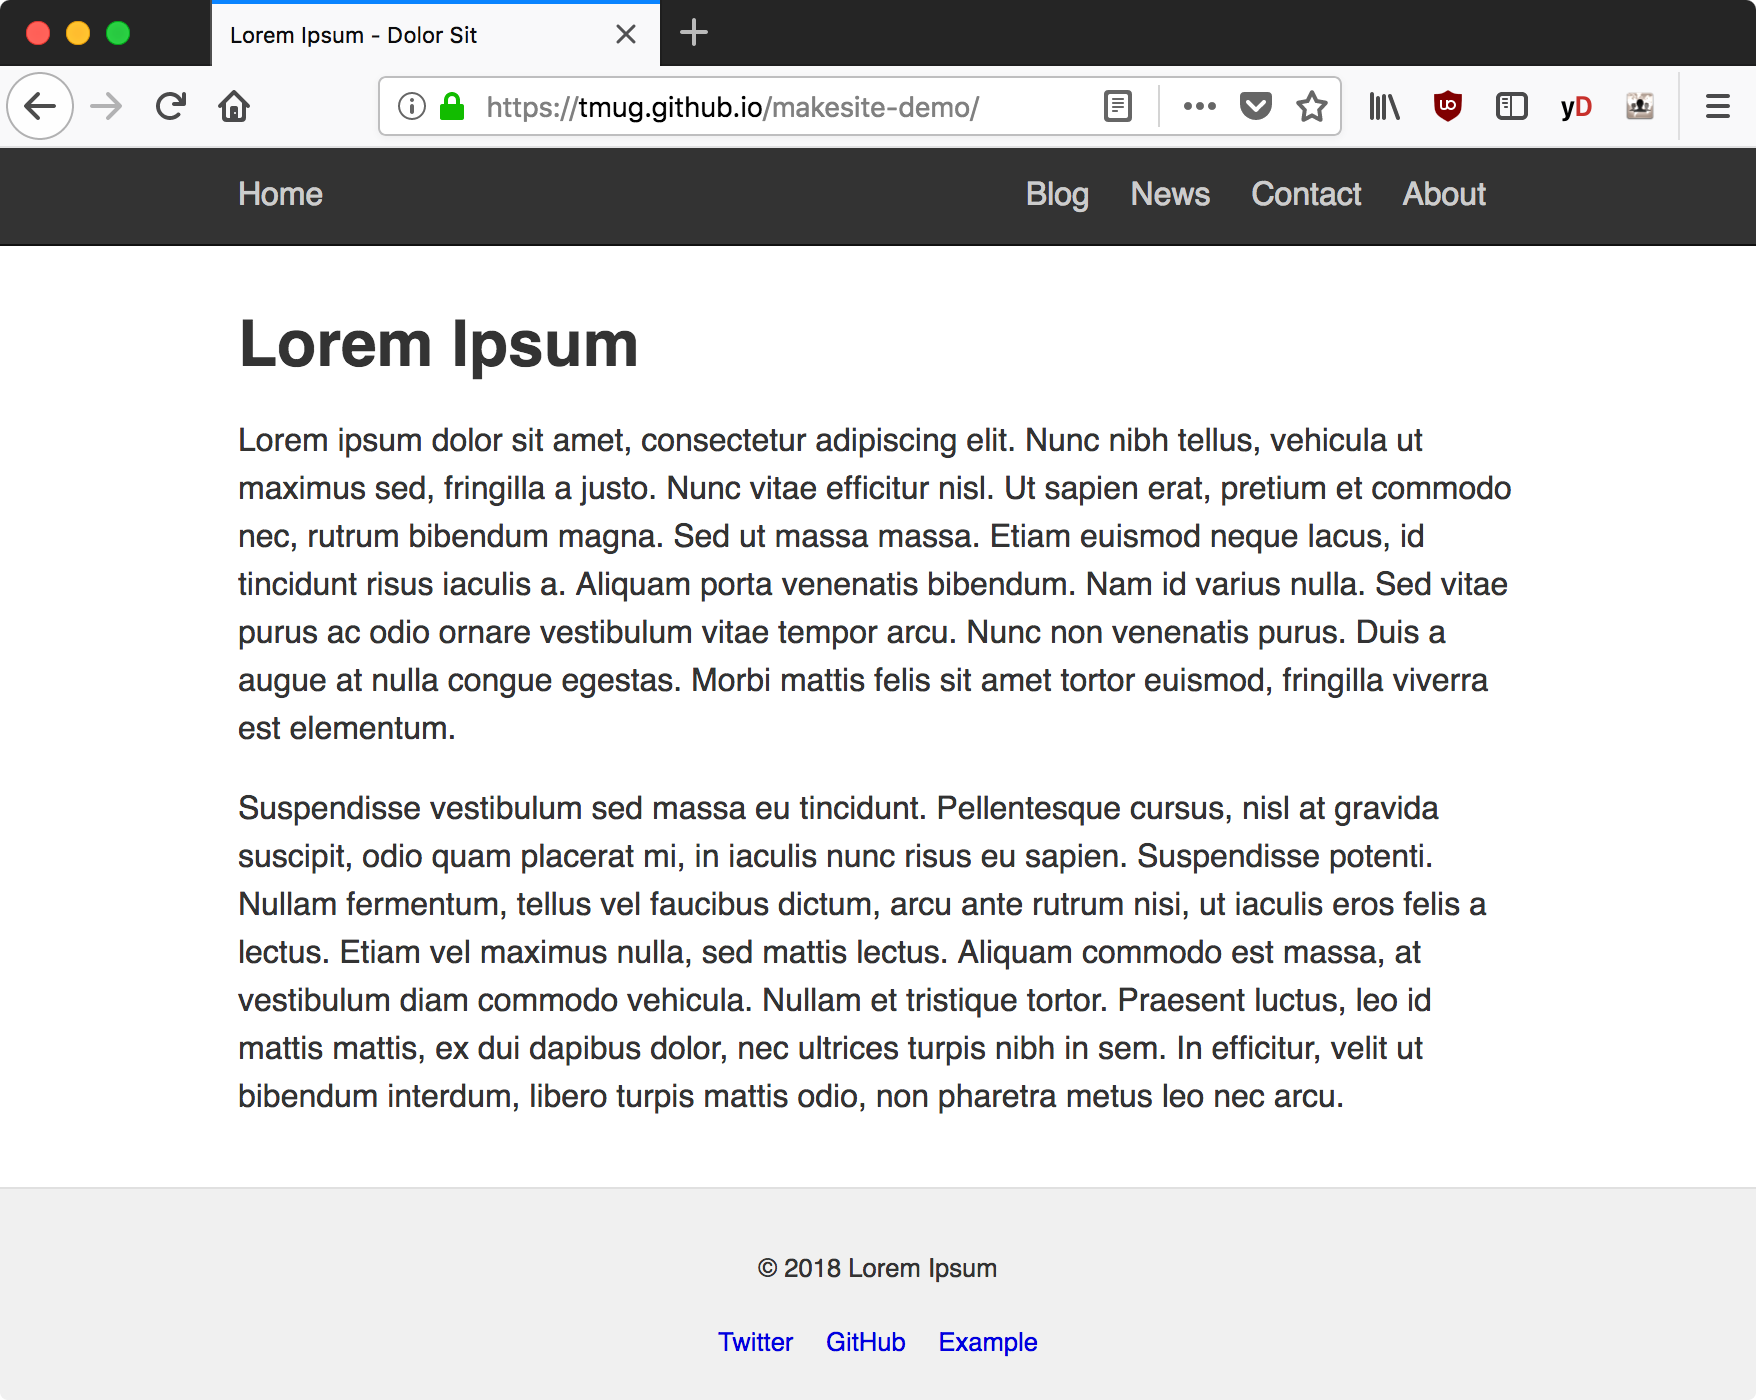
\includegraphics[width=23cm]{makesite-demo-home.png}

    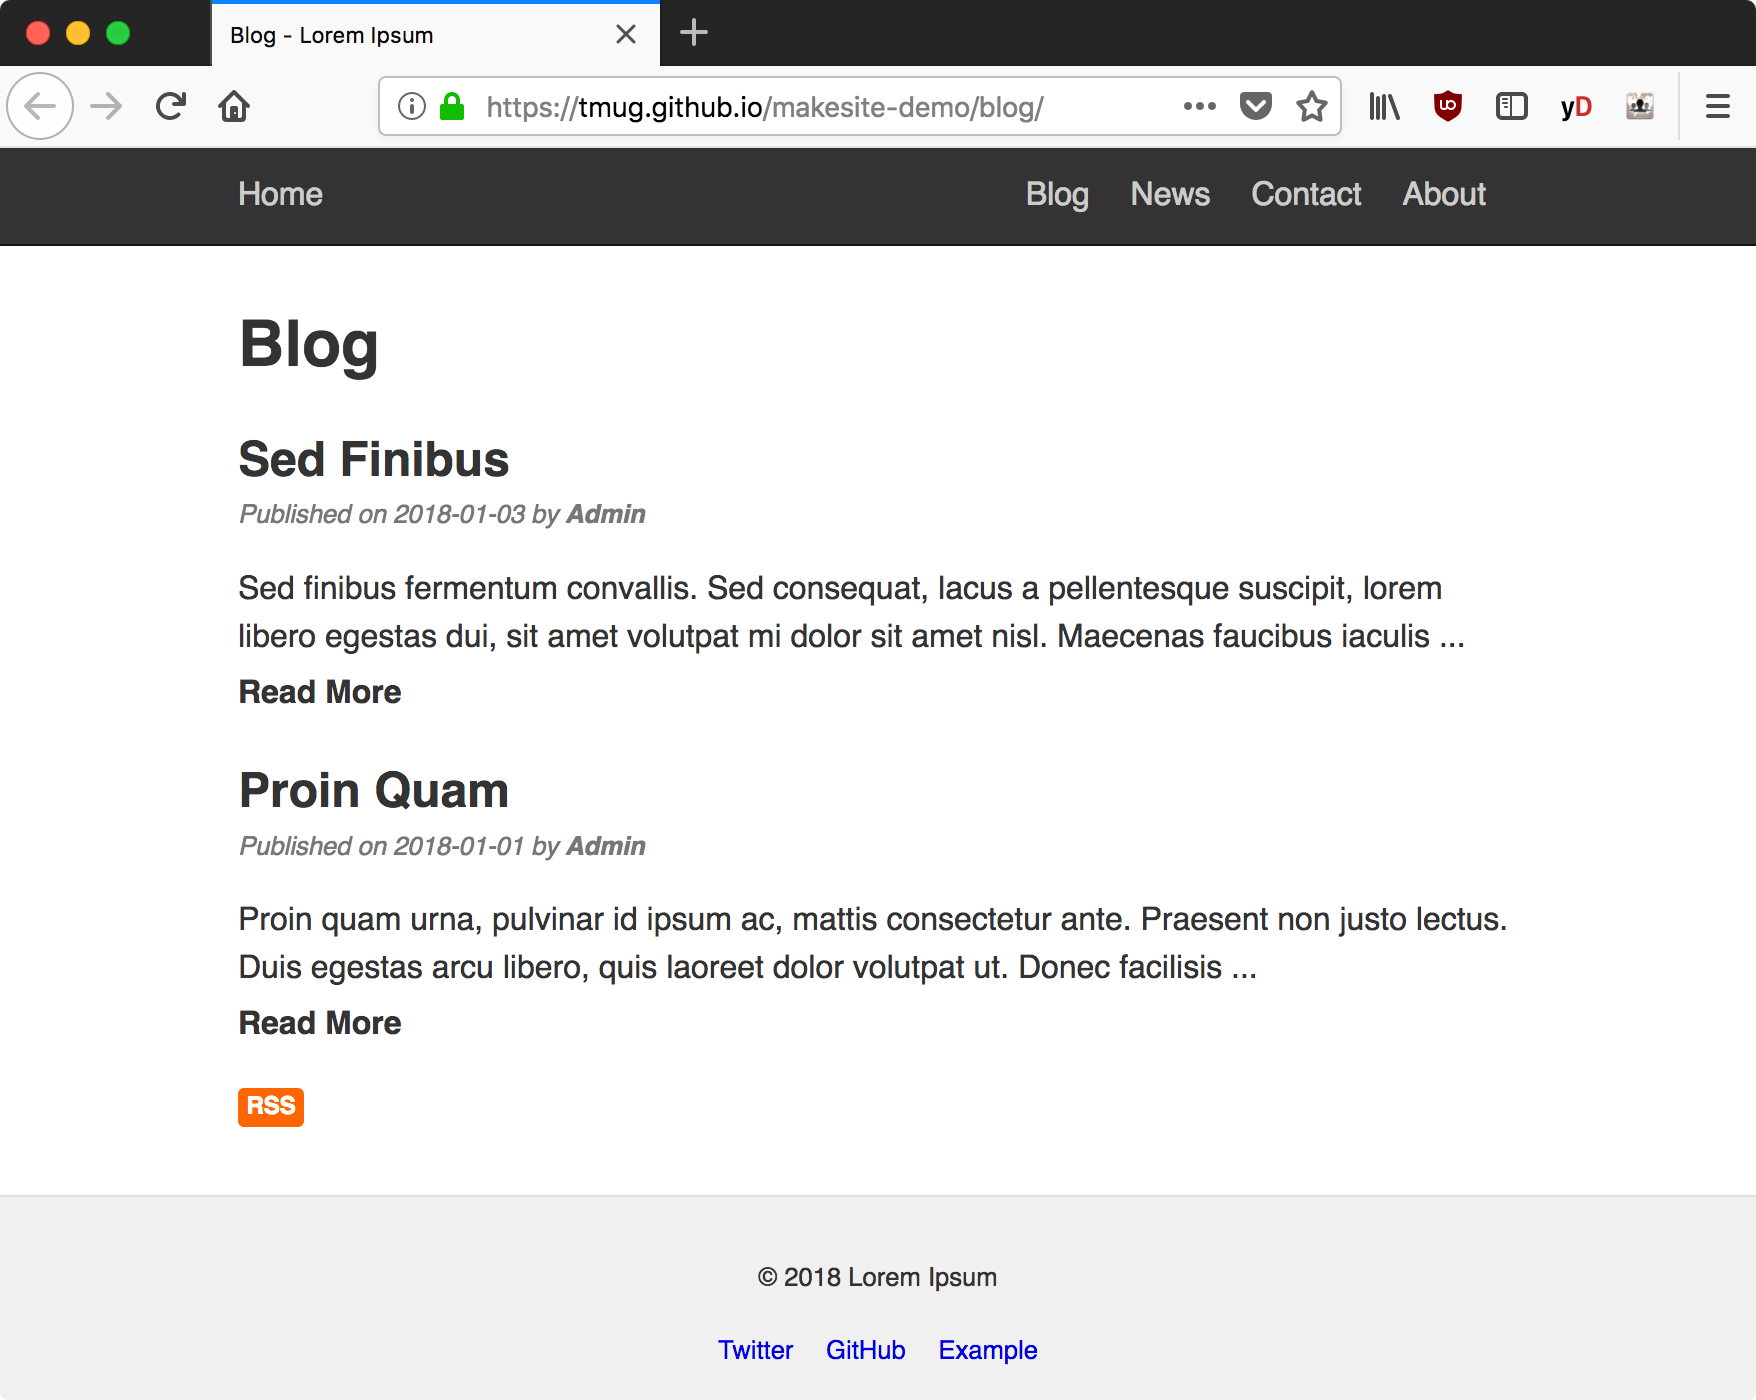
\includegraphics[width=23cm]{makesite-demo-blog.png}

    Demo Short URL: \url{https://git.io/makesite-demo}


    % License
    \color{Navy}
    \section*{License}
    Licensed under the MIT License.

    Go ahead and fork
    \href{https://github.com/sunainapai/makesite}{makesite.py}, replace
    its content with yours, and generate your static website/blog.

\end{multicols}

\end{document}
